\documentclass[8pt, handout=show,notes=show]{beamer}

\usepackage[utf8x]{inputenc}
\usepackage[T1]{fontenc}
\usepackage{wrapfig}
\usepackage{default}
\usetheme[width=2cm]{Goettingen}
\usepackage{amsmath}
\usecolortheme{rose}
\usepackage{enumerate}
\usepackage{graphicx}
\usepackage{wrapfig} 
\usepackage{amsmath}
\usepackage{lmodern}

% \usepackage[colorlinks=true,urlcolor=blue,citecolor=green,linkcolor=blue,bookmarks=true]{hyperref}
\usepackage[french]{babel}
\author[]{Simon Carrignon \\ 
\vfill Encadrant: Nicolas Bred\`{e}che }
\institute[]{
	École~Pratique~des~Hautes~Études, \and TAO/LRI\\
	\pgfdeclareimage[height=0.5cm]{ephe}{../20110616-SoutenanceMemoire/images/logo_ephe_large.jpg} %declare logo image with an alias here 
	\pgfuseimage{ephe} \hfill \pgfdeclareimage[height=0.5cm]{inria}{../20110616-SoutenanceMemoire/images/taologo.jpg} %declare logo image with an alias here 
	\pgfuseimage{inria}
	
}

\usepackage[small]{caption}
% \DeclareLanguageMapping{american}{american-apa}
% \setbeamertemplate{caption}[numbered]
% \usepackage{subcaption}

% \usepackage{tikz}
% \usetikzlibrary{decorations.pathreplacing}
\useoutertheme{infolines}
% \logo{\includegraphics[height=0.5cm]{../20110616-SoutenanceMemoire/images/logo_ephe_large.jpg}}
% 	\usepackage{wrapfig}
\usepackage{subfigure}
\usepackage[footheight=1em]{beamerthemeboxes}

\addfootboxtemplate{\color{black}}{\color{white}
\hspace{2em}Simon Carrignon \hfill\insertframenumber/\inserttotalframenumber\hspace{2em}\null}

\title{Specialization in a swarm of robots using online, onboard, environment driven evolution}

\usepackage{algorithm}
\usepackage{algorithmic}

\usepackage[]{natbib}
\bibpunct{[}{]}{,}{a}{,}{,}
%%Repris du
%%Talk fait a l'EPHE le 16 juin 2011. 
%%Pour presentation du 7 octobre à TAO

\date{$7$ Octobre 2011}
\begin{document}
\begin{frame}
\maketitle

\end{frame}
	\newcommand{\imgSize}{4.2cm}

%%%------------------------------------------------------------------------
%%%----------------------------------------------------------------------
 \section{Embodied evolution in order to design swarms of autonomous agents}
%%%----------------------------------------------------------------------
\begin{frame}{Autonomous agents, swarm intelligence, embodied evolution and the Symbrion project}
        \begin{figure}
		\includegraphics[height=3cm]{../20110616-SoutenanceMemoire/images/symbrion-gc1b.png}
        \end{figure}
	
	Swarm of autonomous agents with limited hardware abilities, in unknown, unpredictable and changing environments. 
	\begin{itemize}
		\item[$\rightarrow$] Goal: open-ended evolution with autonomous agents (online, onboard, distributed).
	\end{itemize}


\end{frame}
%%%----------------------------------------------------------------------
\section{mEDEA}
%%%----------------------------------------------------------------------
\begin{frame}{mEDEA }


\begin{figure}
\includegraphics[height=3cm]{images/medea0}
\end{figure}
mEDEA, unsupervised, distributed evolution :
	\begin{itemize}
		\item Robust to environmental changes [PPSN2010] \nocite{bredeche11mcmds} 
		\item Works in real world [MCMDS2011] %\nocitep{montanier}
		\item Emergence of Altruism [ECAL2011]
	\end{itemize}

\vfill

Motivation : Study specialization and speciation in mEDEA




\end{frame}

%%%----------------------------------------------------------------------
%%%----------------------------------------------------------------------

\section{Speciation}

%%%----------------------------------------------------------------------
%%%----------------------------------------------------------------------

\begin{frame}{Speciation}
\begin{columns}

\column{.65\textwidth}
An old problem since Darwin {\scriptsize \texttt [Darwin1856]} :
\begin{itemize}
	\item allopatric {\scriptsize \texttt [Mayr1942]}
	\item sympatric  {\scriptsize \texttt [MaynardSmith1962] } : a hard way 
	\begin{quotation}
		\small
		[...] if disruptive selection is to lead to stable polymorphism, [..], the conditions which must be satisfied are severe. But they are of a kind which may often be satisfied in laboratory experiments, and wich may perhaps somteimes be met with in Nature.
	\end{quotation}

\end{itemize}


\column{.5\textwidth}
\begin{figure}
	\subfigure[Allopatric speciation]{\includegraphics[width=.3\textwidth]{../20110616-SoutenanceMemoire/images/SpeciationAl}}	\label{figa:specAl} 
	\hspace{.2cm}
	\subfigure[Sympatric speciation]{
		\includegraphics[width=.3\textwidth]{../20110616-SoutenanceMemoire/images/SpeciationSy}
	}	\label{figa:specSy} 
% \caption{Diff. cas}
\end{figure}
\end{columns}


% 			\begin{columns}
% 			 \column{.6\textwidth}

\begin{alertblock}<3->{In a swarm of robot under evolution (sympatric case):}
\begin{itemize}
% 			\centering
\item is speciation possible?
\item in which conditions/mechanismes?
\end{itemize}
\end{alertblock}
% \end{columns}


\end{frame}

%%%----------------------------------------------------------------------
%%%----------------------------------------------------------------------



%%%----------------------------------------------------------------------
%%%----------------------------------------------------------------------

\section{Experiment}

\begin{frame}{Experimental Design}
\begin{columns}[t]


\column{0.45\textwidth}

\begin{block}{The environment:}
\begin{itemize}
\item fixed number of agents,
\item two sources of two kind,
\end{itemize}
\end{block}

\column{0.45\textwidth}

\begin{block}{Ability to forage:}
\begin{itemize}
\item a gene $g_{skill}$ which determine the "foraging skills" of an agent
\end{itemize}

\end{block}

\end{columns}


\begin{columns}


\column{0.57\textwidth}

\begin{block}{The foraging reward function: $F_{rwd}$}

Quantity of energy agent can take :

$F_{rwd,t}(i,Q) = f_{skill}\left(g_{s,i},T_Q\right)\alpha$%\times d_{penality}\left(h_{Q,t}\right)\times \alpha$

\end{block}


\end{columns}
\begin{figure}
\includegraphics[width=.45\textwidth]{../images/sparsityEffect/f_skill}
\end{figure}
\end{frame}
 
%%%----------------------------------------------------------------------
%%%----------------------------------------------------------------------


\begin{frame}{5 topologies}
\begin{table}[h]
\begin{tabular}{l|c|c|}
\small
&robot disposition& resources disposition: \\
\hline
ENV0 &every robot can communicate& Full access\\\hline
ENV1 &Chain & Full access\\\hline
ENV2 &Chain & Limited access \\\hline
ENV3&Two groups & Full access\\\hline
ENV4&Two groups & Limited access 
\end{tabular}
\end{table}
\end{frame}

%%%----------------------------------------------------------------------
%%%----------------------------------------------------------------------

\subsection{5 topologies}
\begin{frame}


\renewcommand{\imgSize}{0.40\textwidth}
\small
\begin{table}[h]
\centering
\begin{tabular}{lcc}
&Full access&Limited access\\
% \newline
all linked&\includegraphics[width=\imgSize]{../images/5StaticEnv/environments/staticEnv0}&\\
% \newline
Chain&\includegraphics[width=\imgSize]{../images/5StaticEnv/environments/staticEnv1}&\includegraphics[width=\imgSize]{../images/5StaticEnv/environments/staticEnv2}\\
Two groups&\includegraphics[width=\imgSize]{../images/5StaticEnv/environments/staticEnv3}&\includegraphics[width=\imgSize]{../images/5StaticEnv/environments/staticEnv4}\\
% \newline
\end{tabular}
\label{tab:gt}

\end{table}%

\end{frame}
%%%----------------------------------------------------------------------
%%%----------------------------------------------------------------------



\subsection{Exhaustive analyse of the density's effect}
\begin{frame}{Density's effect}
\renewcommand{\imgSize}{3cm}
How the density of the communication's network affects speciation?

\vfill
\begin{columns}
\column{0.3\textwidth}
Sparsity = $0.99$

\column{0.3\textwidth}
$0.50$
\column{0.3\textwidth}
$0.02$
\end{columns}
\vfill
\begin{columns}
 \column{0.3\textwidth}
 
\includegraphics[width=\imgSize]{images/networks/neato_Network_sparsity1}\\
 \column{0.3\textwidth}
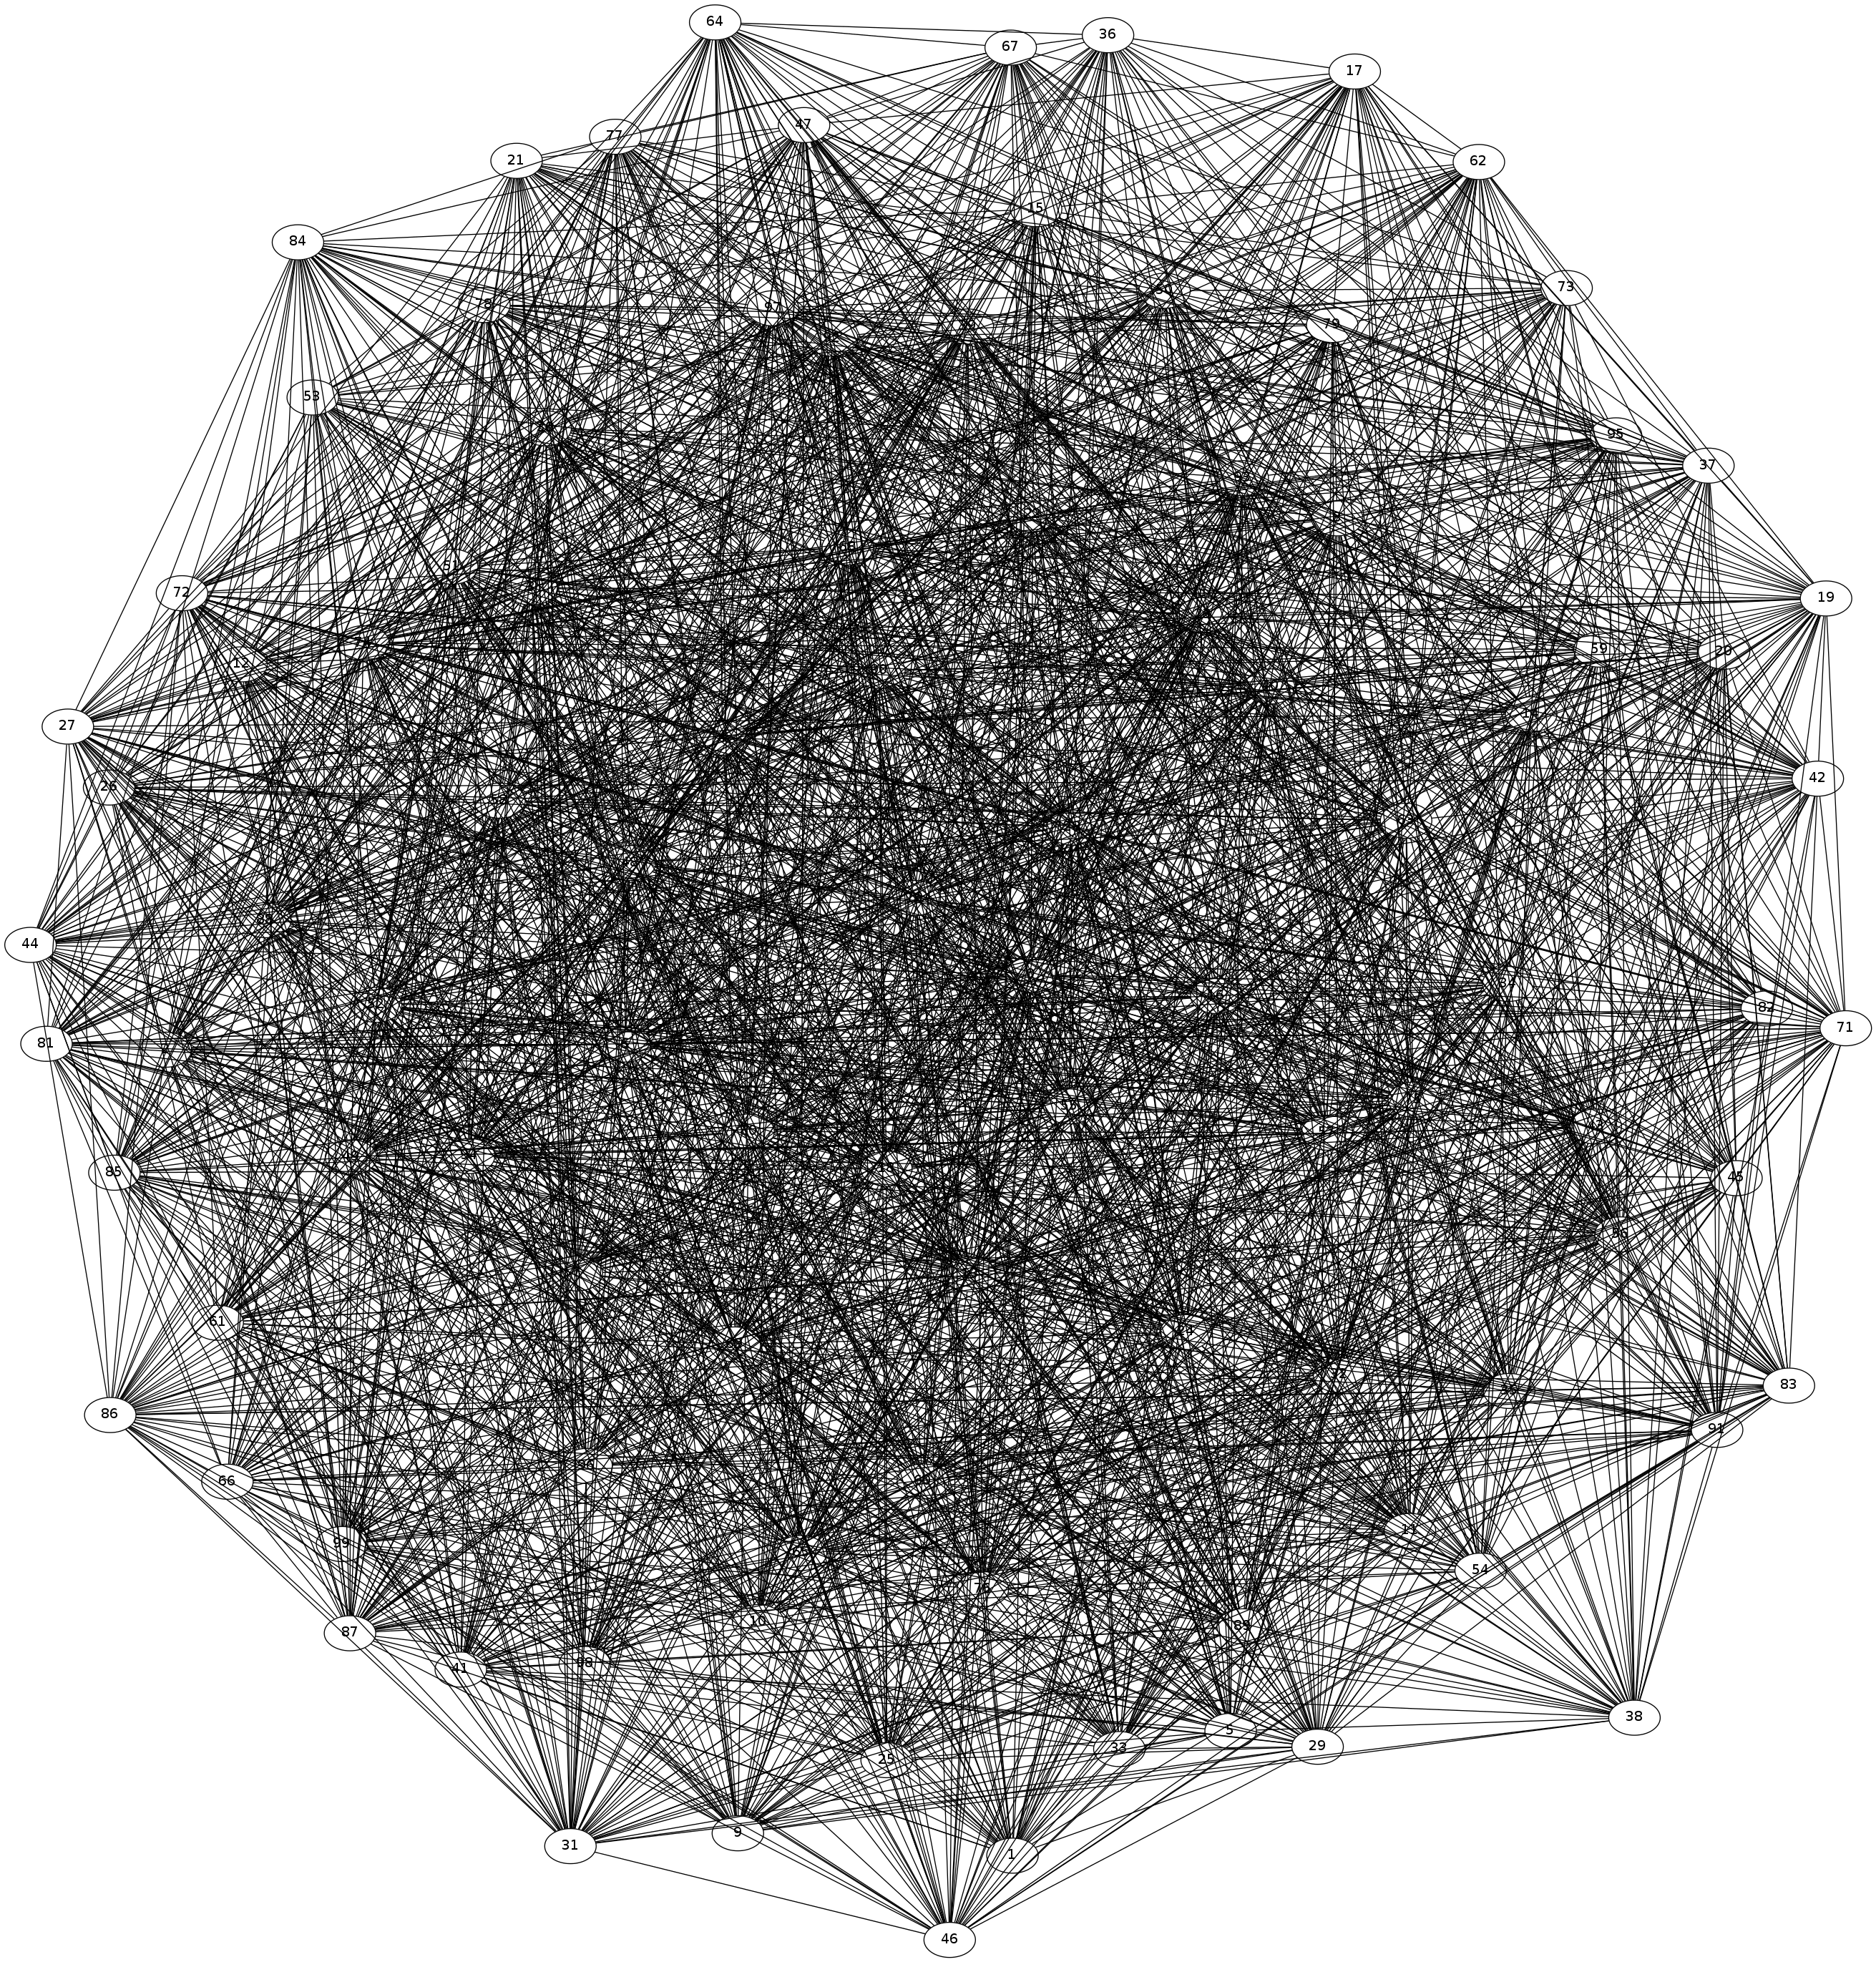
\includegraphics[width=\imgSize]{images/networks/neato_Network_sparsity50.png}\\
 \column{0.3\textwidth}
\includegraphics[width=\imgSize]{images/networks/neato_Network_sparsity98.png}\\
\end{columns}

\end{frame}



%%%----------------------------------------------------------------------
%%%----------------------------------------------------------------------
\section{Results}

\begin{frame}{Results :}
\begin{figure}
 
\end{figure}

\end{frame}
\begin{frame}{Environment 0}



\begin{table}[H]
\begin{tabular}{cc}
\includegraphics[width=\imgSize]{../images/5StaticEnv/environments/staticEnv0}&\includegraphics[width=\imgSize]{../images/5StaticEnv/alive_staticEnv0}\\
\newline
\includegraphics[width=\imgSize]{../images/5StaticEnv/barplotAliveR1AndR2_median_env0_normalized}\\
\end{tabular}
\end{table}
% \vspace{-1cm}
\end{frame}


\begin{frame}{Envronment 0}
\begin{table}[H]
\centering
\begin{tabular}{cc}
\includegraphics[width=\imgSize]{../images/5StaticEnv/Gplot59_staticEnv0}&\includegraphics[width=\imgSize]{../images/5StaticEnv/Gplot59Static_staticEnv0}\\
\newline
\includegraphics[width=\imgSize]{../images/5StaticEnv/Gplot47_staticEnv0}&\includegraphics[width=\imgSize]{../images/5StaticEnv/Gplot47Static_staticEnv0}\\
\end{tabular}


\end{table}
\end{frame}
\begin{frame}{Envronment 0}
\begin{table}[H]
\centering
\begin{tabular}{cc}
 \includegraphics[width=\imgSize]{../images/5StaticEnv/Gplot62_staticEnv0}&\includegraphics[width=\imgSize]{../images/5StaticEnv/Gplot62Static_staticEnv0}\\
 \newline
 \includegraphics[width=\imgSize]{../images/5StaticEnv/Gplot58_staticEnv0}&\includegraphics[width=\imgSize]{../images/5StaticEnv/Gplot58Static_staticEnv0}\\
\end{tabular}


\end{table}
\end{frame}

\begin{frame}{Environment 1}
\begin{table}[H]
\centering
\begin{tabular}{cc}
\includegraphics[width=\imgSize]{../images/5StaticEnv/environments/staticEnv1}&\includegraphics[width=\imgSize]{../images/5StaticEnv/alive_staticEnv1}\\
\newline
\includegraphics[width=\imgSize]{../images/5StaticEnv/barplotAliveR1AndR2_median_env1_normalized}
\end{tabular}
\end{table}
\end{frame}

\begin{frame}{Environment 1}
\begin{table}[H]
\centering
\begin{tabular}{cc}
\includegraphics[width=\imgSize]{../images/5StaticEnv/Gplot47_staticEnv1}&\includegraphics[width=\imgSize]{../images/5StaticEnv/Gplot47Static_staticEnv1}\\
\newline
\includegraphics[width=\imgSize]{../images/5StaticEnv/Gplot66_staticEnv1}&\includegraphics[width=\imgSize]{../images/5StaticEnv/Gplot66Static_staticEnv1}\\
\end{tabular}

\end{table}
\end{frame}

\begin{frame}{Environment 1}
\begin{table}[H]
\centering
\begin{tabular}{cc}
 \newline
 \includegraphics[width=\imgSize]{../images/5StaticEnv/Gplot29_staticEnv1}&\includegraphics[width=\imgSize]{../images/5StaticEnv/Gplot29Static_staticEnv1}\\
 \newline
 \includegraphics[width=\imgSize]{../images/5StaticEnv/Gplot9_staticEnv1}&\includegraphics[width=\imgSize]{../images/5StaticEnv/Gplot9Static_staticEnv1}\\
\end{tabular}

\end{table}
\end{frame}


\begin{frame}{Environment 2}
 

\begin{table}[H]
\centering
\begin{tabular}{cc}
\includegraphics[width=\imgSize]{../images/5StaticEnv/environments/staticEnv2}&\includegraphics[width=\imgSize]{../images/5StaticEnv/alive_staticEnv2}\\
\newline
\includegraphics[width=\imgSize]{../images/5StaticEnv/barplotAliveR1AndR2_median_env2_normalized}

\end{tabular}
\end{table}
\end{frame}

\begin{frame}{Environment 2}
\begin{table}[H]
\centering
\begin{tabular}{cc}
\includegraphics[width=\imgSize]{../images/5StaticEnv/Gplot22_staticEnv2}&\includegraphics[width=\imgSize]{../images/5StaticEnv/Gplot22Static_staticEnv2}\\
\newline
\includegraphics[width=\imgSize]{../images/5StaticEnv/Gplot66_staticEnv2}&\includegraphics[width=\imgSize]{../images/5StaticEnv/Gplot66Static_staticEnv2}\\
\end{tabular}

\end{table}
\end{frame}
\begin{frame}{Environment 2}
\begin{table}[H]
\centering
\begin{tabular}{cc}
 \includegraphics[width=\imgSize]{../images/5StaticEnv/Gplot5_staticEnv2}&\includegraphics[width=\imgSize]{../images/5StaticEnv/Gplot5Static_staticEnv2}\\
 \newline
 \includegraphics[width=\imgSize]{../images/5StaticEnv/Gplot92_staticEnv2}&\includegraphics[width=\imgSize]{../images/5StaticEnv/Gplot92Static_staticEnv2}\\
\end{tabular}

\end{table}
\end{frame}

\begin{frame}{Environment 3}

\begin{table}[H]
\centering
\begin{tabular}{cc}
\includegraphics[width=\imgSize]{../images/5StaticEnv/environments/staticEnv3}&\includegraphics[width=\imgSize]{../images/5StaticEnv/alive_staticEnv3}\\
\newline
\includegraphics[width=\imgSize]{../images/5StaticEnv/barplotAliveR1AndR2_median_env3_normalized}
\end{tabular}

\end{table}
\end{frame}

\begin{frame}{Environment 3}

\begin{table}[H]
\centering
\begin{tabular}{cc}
\includegraphics[width=\imgSize]{../images/5StaticEnv/Gplot5_staticEnv3}&\includegraphics[width=\imgSize]{../images/5StaticEnv/Gplot5Static_staticEnv3}\\
\newline
\includegraphics[width=\imgSize]{../images/5StaticEnv/Gplot8_staticEnv3}&\includegraphics[width=\imgSize]{../images/5StaticEnv/Gplot8Static_staticEnv3}\\

\end{tabular}

\end{table}
\end{frame}

\begin{frame}{Environment 3}

\begin{table}[H]
\centering
\begin{tabular}{cc}
 \includegraphics[width=\imgSize]{../images/5StaticEnv/Gplot51_staticEnv3}&\includegraphics[width=\imgSize]{../images/5StaticEnv/Gplot51Static_staticEnv3}\\
 \newline
 \includegraphics[width=\imgSize]{../images/5StaticEnv/Gplot99_staticEnv3}&\includegraphics[width=\imgSize]{../images/5StaticEnv/Gplot99Static_staticEnv3}\\
\end{tabular}

\end{table}
\end{frame}


\begin{frame}{Environment 4}

\begin{table}[H]
\centering
\begin{tabular}{cc}
\includegraphics[width=\imgSize]{../images/5StaticEnv/environments/staticEnv4}&\includegraphics[width=\imgSize]{../images/5StaticEnv/alive_staticEnv4}\\
\newline
\includegraphics[width=\imgSize]{../images/5StaticEnv/barplotAliveR1AndR2_median_env4_normalized}
\end{tabular}
\end{table}
\end{frame}


\begin{frame}{Environment 4}
\begin{table}[H]
\centering
\begin{tabular}{cc}
\includegraphics[width=\imgSize]{../images/5StaticEnv/Gplot17_staticEnv4}&\includegraphics[width=\imgSize]{../images/5StaticEnv/Gplot17Static_staticEnv4}\\
\newline
\includegraphics[width=\imgSize]{../images/5StaticEnv/Gplot40_staticEnv4}&\includegraphics[width=\imgSize]{../images/5StaticEnv/Gplot40Static_staticEnv4}\\
\end{tabular}

\end{table}
\end{frame}

\begin{frame}{Environment 4}
\begin{table}[H]
\centering
\begin{tabular}{cc}
 \includegraphics[width=\imgSize]{../images/5StaticEnv/Gplot62_staticEnv4}&\includegraphics[width=\imgSize]{../images/5StaticEnv/Gplot62Static_staticEnv4}\\
 \newline
 \includegraphics[width=\imgSize]{../images/5StaticEnv/Gplot58_staticEnv4}&
\end{tabular}

\end{table}
\end{frame}


\begin{frame}{Effect of the sparsity}
\renewcommand{\imgSize}{3.8cm}

\begin{table}[H]
% \caption{pourcentage }
\centering
\begin{tabular}{cc}
R1 & R0\\
 \includegraphics[width=\imgSize]{images/R1_median}&\includegraphics[width=\imgSize]{images/R0_median}\\
 \includegraphics[width=\imgSize]{images/active_median}\\
 Number of alive
\end{tabular}

\end{table}

\begin{figure}
alive
\center
\end{figure}
\end{frame}

\renewcommand{\imgSize}{4cm}

\begin{frame}{slice through the $Q_{r1}$'s availablities axis : }
\begin{figure}[H]
\includegraphics[width=\imgSize]{images/alive_density_r1-50.png}
\includegraphics[width=\imgSize]{images/alive_density_r1-70.png}\\
\includegraphics[width=\imgSize]{images/alive_density_r1-90.png}
\includegraphics[width=\imgSize]{images/active_median}
\end{figure}

\end{frame}
\begin{frame}{slice through the $Q_{r1}$'s availablities axis : }

\begin{figure}[H]
\includegraphics[width=\imgSize]{images/harvestr1_density_r1-50.png}
\includegraphics[width=\imgSize]{images/harvestr1_density_r1-70.png}\\
\includegraphics[width=\imgSize]{images/harvestr1_density_r1-90.png}
\includegraphics[width=\imgSize]{images/R1_median}
\end{figure}
\end{frame}

\begin{frame}{ slice through the density axis : }
\begin{figure}[H]
\includegraphics[width=\imgSize]{images/alive_r1_density-2.png}
\includegraphics[width=\imgSize]{images/alive_r1_density-8.png}\\
\includegraphics[width=\imgSize]{images/alive_r1_density-60.png}
\includegraphics[width=\imgSize]{images/active_median}

\end{figure}
\end{frame}

\begin{frame}{ slice through the density axis : }
\begin{figure}[H]
\includegraphics[width=\imgSize]{images/harvestr1_r1_density-2.png}
\includegraphics[width=\imgSize]{images/harvestr1_r1_density-8.png}\\
\includegraphics[width=\imgSize]{images/harvestr1_r1_density-60.png}
\includegraphics[width=\imgSize]{images/R1_median}

\end{figure}
\end{frame}
%%%----------------------------------------------------------------------
%%%----------------------------------------------------------------------
%%%----------------------------------------------------------------------
\begin{frame}%\addtocounter{framenumber}{-1}
\begin{center}
Merci pour votre attention.
\end{center}
\end{frame}


\end{document}
		
